
%(BEGIN_QUESTION)
% Copyright 2012, Tony R. Kuphaldt, released under the Creative Commons Attribution License (v 1.0)
% This means you may do almost anything with this work of mine, so long as you give me proper credit

Anta at du blir bedt om å utføre en ``utløsertest'' av høytemperatur-nedstengningene i dette naturgass-kompressorsystemet. Du må teste både motorens og kompressorens høytemperatur-utløsningsfunksjon. Testene skal være så grundige og realistiske som mulig, men uten å stoppe komprimeringen av naturgass.

$$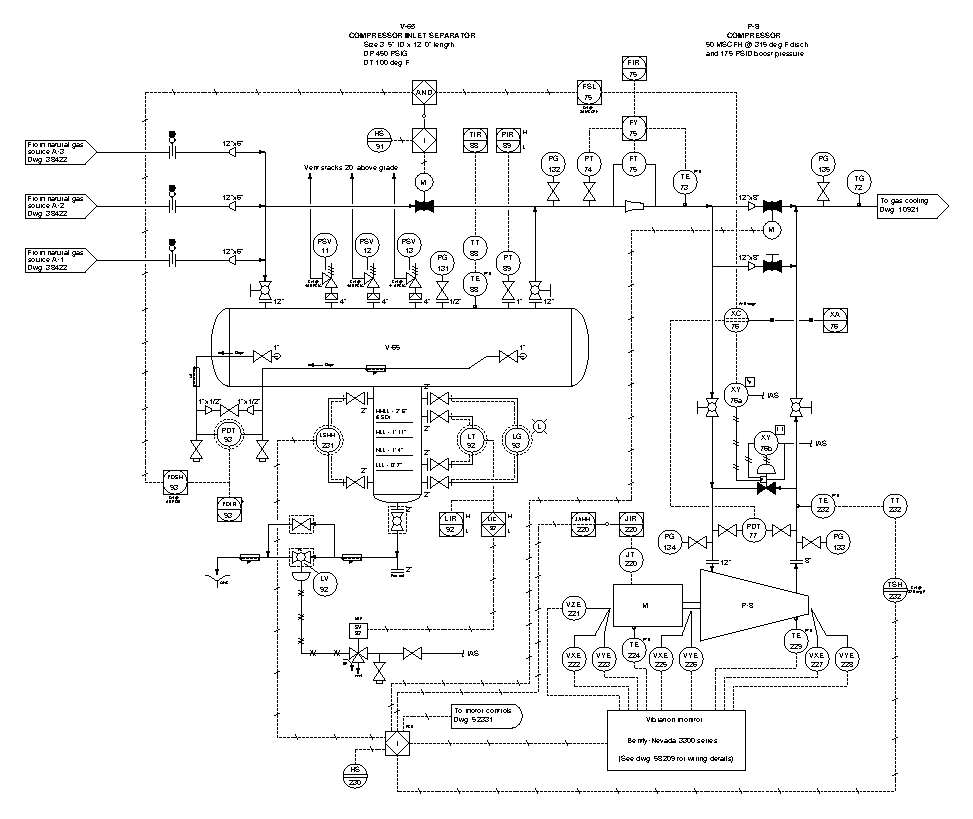
\includegraphics[width=15.5cm]{i0003rx01.eps}$$

Forklar hvordan du ville simulert en høytemperaturtilstand, og hvordan du ville verifisert korrekt funksjon av nødavstengningssystemet (ESD) uten at kompressoren faktisk stopper.

\vskip 20pt \vbox{\hrule \hbox{\strut \vrule{} {\bf Forslag til sokratisk diskusjon} \vrule} \hrule}

\begin{itemize}
\item{} Basert på diagrammet, forklar formålet med nødavstengningssystemet. Hvilke konkrete betingelser overvåkes for utløsning, og hva er konsekvensene av en utløsning?
\end{itemize}

\underbar{file i01242}
%(END_QUESTION)





%(BEGIN_ANSWER)

Simuleringshint: temperatursensorene er {\it RTD-er}.

%(END_ANSWER)





%(BEGIN_NOTES)

Ved å koble et potensiometer i stedet for RTD-en kan du simulere ønsket temperaturtilstand. For å unngå faktisk stopp av kompressorsystemet må du deaktivere/frakoble bypassventilen samt motorstyringene vist i tegning 52331. Deretter bruker du instrumentmåling for å verifisere at riktige ``utløsning''-signaler sendes til de deaktiverte sluttkontrollelementene under testen.




\vskip 20pt \vbox{\hrule \hbox{\strut \vrule{} {\bf Virtuell feilsøking} \vrule} \hrule}

Denne oppgaven egner seg godt som en ``Virtuell feilsøking''-øvelse. Når du presenterer diagrammet for elevene, tenker du først ut en bestemt feil i systemet. Deretter presenterer du ett eller flere symptomer på denne feilen (noe en operatør eller annen bruker av systemet kan observere). Elevene foreslår deretter ulike diagnostiske tester på systemet for å identifisere type feil og hvor den sitter, som om de var teknikere som feilsøker problemet. Din oppgave er å fortelle hva resultatet ville vært for hver foreslåtte diagnostiske test, og dokumentere resultatene slik at alle elevene kan se dem.

Under og etter øvelsen er det nyttig å stille oppfølgingsspørsmål til elevene, for eksempel:

\begin{itemize}
\item{} Hva forteller resultatet av den siste diagnostiske testen deg om feilen?
\item{} Anta at resultatet av den siste diagnostiske testen var annerledes. Hva ville det i så fall fortalt deg om feilen?
\item{} Er den siste diagnostiske testen den beste vi kunne gjort?
\item{} Hva ville vært den ideelle rekkefølgen på testene for å diagnostisere problemet med færrest mulig trinn?
\end{itemize}

\vskip 20pt \vbox{\hrule \hbox{\strut \vrule{} {\bf Virtuell utløsertesting} \vrule} \hrule}

Denne oppgaven egner seg godt som en ``Virtuell utløsertesting''-øvelse. Når du presenterer diagrammet for elevene, gir du en oppgave der de må finne ut hvordan en komponent kan testes for å verifisere at systemet stopper som det skal ved en unormal (utløsning-)tilstand, under en realistisk begrensning (f.eks. at strømmen til lasten ikke kan kobles ut). Elevene foreslår deretter ulike metoder for å gjennomføre testen. Din oppgave er å avgjøre om de foreslåtte testene vil gi ønsket resultat.

Under og etter øvelsen er det nyttig å stille oppfølgingsspørsmål til elevene, for eksempel:

\begin{itemize}
\item{} Hvor kan den planlagte teststrategien slå feil? Med andre ord: hva kan skje som ødelegger testen, enten ved å gjøre resultatene ugyldige eller ved å bryte de oppgitte begrensningene?
\item{} Anta at begrensningen var annerledes. Hvordan ville det påvirke evnen vår til å gjennomføre testen?
\item{} Er den siste teststrategien den beste vi kunne gjennomført?
\end{itemize}


%INDEX% Prosess: innløpsseparator for gasskompressor (realistisk P&ID vist)
%INDEX% Safety, shutdown system: utløsning testing

%(END_NOTES)
